\documentclass[cjk,slidestop,compress,mathserif,blue]{beamer}
%dvipdfm选项是关键,否则编译统统通不过
%beamer的颜色选项定义的是导航条和标题的颜色(即关键词structure的颜色)

%%%%%%%%%%%%%%%%仅限于XeTeX可使用的宏包%%%%%%%%%%%%%%%%%%%%%%%%%%%%
\usepackage{fontspec,xunicode,xltxtra,beamerthemesplit}
%\usepackage{beamerthemesplit}
\usepackage{xeCJK}
\setCJKmainfont[BoldFont=黑体, ItalicFont=楷体, BoldItalicFont=仿宋]{黑体}
%\setsansfont[Mapping=tex-text]{Adobe 黑体 Std}
%如果装了Adobe Acrobat,可在font.conf中配置Adobe字体的路径以使用其中文字体
%也可直接使用系统中的中文字体如SimSun,SimHei,微软雅黑 等
%原来beamer用的字体是sans family;注意Mapping的大小写,不能写错

%%%%%%%%   确定标题和导航条结构的框架     %%%%%%%%%%%%
\usepackage{beamerthemeshadow}                       %
%\usepackage{beamerthemeclassic}%导航条色与背景色一致%
%%%%%%%%%%%%%%%%%%%%%%%%%%%%%%%%%%%%%%%%%%%%%%%%%%%%%%
\setbeamerfont{roman title}{size={}}
%\usepackage{CJK} % CJK 中文支持                                  %
\usepackage{amsmath,amsthm,amsfonts,amssymb,bm}
\usepackage{mathrsfs}
\usepackage{xcolor}                                        %使用默认允许使用颜色
\usepackage{hyperref} 
\usepackage{graphicx}
\usepackage{subfigure}           %图片跨页

%\usepackage[numbers,sort&compress]{natbib} %紧密排列             %
\usepackage[sectionbib]{chapterbib}        %每章节单独参考文献   %
\usepackage{hypernat}                                                                         %
%\usepackage[dvipdfm,bookmarksopen=true,pdfstartview=FitH,CJKbookmarks]{hyperref}		%
\hypersetup{bookmarksnumbered,colorlinks,linkcolor=brown,citecolor=blue,urlcolor=red}         %
%参考文献含有超链接引用时需要下列宏包,注意与natbib有冲突        %
%\usepackage[dvipdfm]{hyperref}                                  %
%\usepackage{hypernat}                                           %
\newcommand{\upcite}[1]{\hspace{0ex}\textsuperscript{\cite{#1}}} %

%\useoutertheme{smoothbars}
\useinnertheme[shadow=true]{rounded}
\usetheme{Berkeley}                                          %主题式样
%\usetheme{Luebeck}

\usecolortheme{lily}                                        %颜色主题式样

\usefonttheme{professionalfonts}                           %字体主题样式宏包

%\beamertemplatetransparentcoveredhigh                      %使所有被隐藏的文本高度透明
\beamertemplatetransparentcovereddynamicmedium             %使所有被隐藏的文本完全透明,动态,动态的范围很小
\mode<presentation>
%\beamersetaveragebackground{gray}                          %设置背景颜色(单一色) 
\beamertemplateshadingbackground{green!10}{red!5}         %设置背景颜色(渐变色)

%i放置单位logo
%\logo{
\includegraphics[width=1.6cm,height=0.35cm]{Figures/BCC_logo-1.png}}	%简单设置logo

%\pgfdeclareimage[width=3.5cm]{logoname}{Figures/BCC_logo-1.png}		%logo置于左侧微调
%\logo{\pgfuseimage{logoname}{\vspace{0.2cm}\hspace*{-2.0cm}}}

%在指定位置精确放置logo
\usepackage{tikz}
\usepackage{beamerfoils}
\usepackage{pgf}
\logo{\pgfputat{\pgfxy(11.68,0.15)}{
\includegraphics[height=1.01cm,viewport=0 0 140 120,clip]{Figures/BCC_logo-1.png}}\pgfputat{\pgfxy(10.502,-0.218)}{
\includegraphics[height=0.369cm,viewport=140 0 540 120,clip]{Figures/BCC_logo-1.png}}}
%\logo{\pgfputat{\pgfxy(11.68,0.15)}{
\includegraphics[height=0.95cm,viewport=0 0 510 360,clip]{Figures/Logo_Gainstrong.png}}\pgfputat{\pgfxy(10.333,-0.195)}{
\includegraphics[height=0.35cm,viewport=530 70 1100 218,clip]{Figures/Logo_Gainstrong.png}}}
%\MyLogo{
%	\pgfputat{\pgfxy(-50,-50)}{\pgfbox[right,base]{
\includegraphics[height=1cm]{Figures/BCC_logo-1.png}}}

%logo作为背景放置
%\setbeamertemplate{background}{
%	\pgfputat{\pgfxy(6.5,-0.5)}{\pgfbox[left,top]{\pgfimage[height=1.1cm]{Figures/BCC_logo-1.png}}}}

%\logo{}									%不显示logo

\begin{document}
%\begin{CJK*}{GBK}{song}
%\begin{CJK*}{GBK}{kai}
%beamer下不能用\songyi、\zihao等命令!
%\graphicspath{Figures/}

%-------------------------------PPT Title-------------------------------------
\title{旋-轨耦合与非共线磁矩}
%-----------------------------------------------------------------------------

%----------------------------Author & Date------------------------------------
\author{北京市计算中心\;云平台\:姜骏}
\date{\textrm{2016.11.30}}
%\date{2013.09.10}
\frame{\titlepage}
%-----------------------------------------------------------------------------

%------------------------------------------------------------------------------列出全文 outline ---------------------------------------------------------------------------------
\section*{}
\frame[allowframebreaks]
{
  \frametitle{Outline}
%  \frametitle{\textcolor{mycolor}{\secname}}
  \tableofcontents%[current,currentsection,currentsubsection]
}
%在每个section之前列出全部Outline
%类似的在每个subsection之前列出全部Outline是\AtBeginSubsection[]
\AtBeginSection[]
{
  \frame<handout:0>
  {
    \frametitle{Outline}
%全部Outline中,本部分加亮
    \tableofcontents[current,currentsection]
  }
}

%------------------------------------------------------------------------------PPT main Body------------------------------------------------------------------------------------
\small
\section{旋-轨耦合作用的本质}
\frame
{
\frametitle{旋-轨耦合的起源}
\begin{itemize}
	\item 电场对静止的电荷有静电力作用(\textrm{Coulomb}力)
	\item 电场对运动的电荷除静电力外还有磁场力作用
	\item 磁场对运动的电荷有力的作用(\textrm{Lorentz}力)
\end{itemize}
自旋-轨道耦合本质:~\textcolor{red}{外电场对运动自旋磁矩的作用,是相对论效应}
\begin{figure}[h!]
\centering
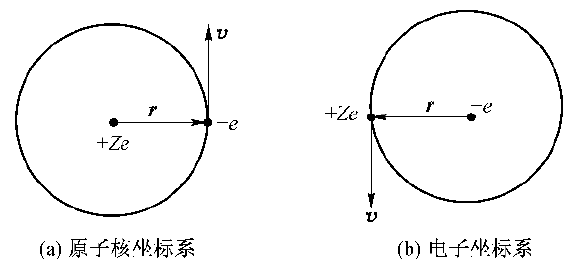
\includegraphics[height=1.15in,width=2.45in,viewport=0 0 600 270,clip]{Figures/SOC_cor.png}
\caption{\small \textrm{A schematic coordinate for an electron in atom: (a) atomic coordinate system, (b) electron coordinate ones.}}%(与文献\cite{EPJB33-47_2003}图1对比)
\label{Muffin_tin}
\end{figure}
}

\frame
{
	\frametitle{经典唯象的旋-轨耦合}
	\begin{itemize}
		\item 在原子核坐标系下,根据\textrm{Coulomb}定理,运动电子-$e$的速度$v$~,并有自旋磁矩,离子实的势场会与运动的磁矩发生相互作用
		\item 由于运动是相对的,在电子坐标系下,选-轨耦合可理解为电场$\vec E$以速度-$v$运动产生磁场$\vec B$,磁场会对电子自旋有力的作用
	\end{itemize}
	\begin{displaymath}
		\vec B=\frac{\mu_0\vec j\times\vec r}{r^3}=\mu_0\varepsilon_0(\vec v\times\vec E)
	\end{displaymath}
其中$\vec v$是电子运动速度,$\vec E$是离子实在电子处的电场。根据电场强度的径向分布形式
\begin{displaymath}
	\vec E=\frac1{e}\frac{\partial V}{\partial r}\frac{\vec r}r
\end{displaymath}
利用轨道角动量关系$\vec L=\vec r\times\vec p$和$\vec p=m\vec v$,可得磁感应强度
\begin{displaymath}
	\vec B=\frac1{emc^2}\frac1r\frac{\partial V}{\partial r}\vec L
\end{displaymath}
}

\frame
{
	\frametitle{经典唯象的旋-轨耦合}
对自由电子自旋,离子实在电子处的磁场对\textrm{Hamiltonian}贡献为
\begin{displaymath}
	\vec H=\frac{(\vec{\sigma}\cdot\vec p)^2}{2m}
\end{displaymath}

考虑磁场与交变电磁场$\mathbf{A}$:~$\vec B=\nabla\times\mathbf A$,因此
\begin{displaymath}
	H=\frac{\left( \vec{\sigma}\cdot\left( \vec p+\dfrac ec\mathbf A \right) \right)^2}{2m}
\end{displaymath}
利用关系式$(\vec{\sigma}\cdot\mathbf A)(\vec{\sigma}\cdot\mathbf B)=\mathbf{A}\cdot\mathbf{B}+\mathrm{i}\vec{\sigma}(\mathbf{A}\times\mathbf{B})$,可得
\begin{displaymath}
	H=\frac{\left( \vec p+\frac ec\mathbf{A} \right)^2}{2m}+\underline{\textcolor{red}{\frac{\mathrm i}{2m}\vec{\sigma}\cdot\left( \vec p+\frac ec\mathbf{A} \right)\times\left( \vec p+\frac ec\mathbf{A} \right)}}
\end{displaymath}
其中第一项是轨道磁矩与外磁场相互作用,第二项是自旋磁矩与外磁场相互作用
}

\frame
{
	\frametitle{经典唯象的旋-轨耦合}
	自旋磁矩与外场相互作用
	\begin{displaymath}
		\begin{aligned}
			&\frac{\mathrm{i}e}{2mc}\vec{\sigma}\cdot[(\vec p\times\mathbf{A})+(\mathbf{A})\times\vec p]=\frac{\mathrm{i}e}{2mc}\vec{\sigma}\cdot(-\mathrm{i}\hbar\nabla\times\mathbf{A})\\
			=&\frac{eh}{2mc}\vec{\sigma}\cdot\mathbf{B}=-\vec{\mu}_s\cdot\mathbf{B}
		\end{aligned}
	\end{displaymath}
	其中$\vec \mu_s=-g_s\mu_B\vec S$是电子自旋$\vec S$磁矩,$g_s$是电子自旋$g$因子,$\mu_B$是\textrm{Bohr}磁子,$\vec S$是自旋角动量,因此可得自旋-轨道相互作用能量为:
	\begin{displaymath}
		\begin{aligned}
			U=&\frac1{m^2c^2}\frac1r\frac{\partial V}{\partial r}\vec L\cdot\vec S\\
			=&-\frac1{m^2c^2}\nabla V\cdot(\vec S\times\vec p)
		\end{aligned}
	\end{displaymath}
	考虑电子参照系的非惯性系性质,会产生\textrm{Thomas}进动,因此非惯性系中真空自旋-轨道耦合\textrm{Hamiltonian}为
	\begin{displaymath}
		\vec H_{\mathrm{SO}}=-\frac1{4m^2c^2}(\vec{\sigma\cdot\vec p})\times\nabla V
	\end{displaymath}
}

\frame
{
	\frametitle{由\textrm{Dirac~}方程导出}
	自旋是相对量量子力学的自然结果,严格地给出自旋-轨道耦合必须要从\textrm{Dirac~}方程出发,由\textrm{Dirac~}方程的非相对论极限可得到旋-轨耦合的具体形式,由\textrm{Dirac~}算符
	\begin{displaymath}
		\vec H_{\mathrm D}=c\vec{\alpha}\cdot\vec p+(\vec{\beta}-1)mc^2+V(\vec r)
	\end{displaymath}
	其中$\mathbf{\alpha}$和$\mathbf{\beta}$是$4\times4$的矩阵
	\begin{displaymath}
		\vec{\alpha}=\left(
		\begin{matrix}
			0 &\vec{\sigma}\\
			\vec{\sigma} &0
		\end{matrix}
		\right)\quad\beta=\left(
		\begin{matrix}
			1 &0 &0 &0\\
			0 &1 &0 &0\\
			0 &0 &-1 &0\\
			0 &0 &0 &-1
		\end{matrix}
		\right)
	\end{displaymath}
	$\vec{\sigma}$是\textrm{Pauli-spin~}矩阵,
	\begin{displaymath}
		\sigma_x=\left( 
		\begin{matrix}
			0 &1\\
			1 &0
		\end{matrix}
		\right)\quad
		\sigma_y=\left( 
		\begin{matrix}
			0 &-\mathrm{i}\\
			\mathrm{i} &0
		\end{matrix}
		\right)\quad
		\sigma_z=\left( 
		\begin{matrix}
			1 &0\\
			0 &-1
		\end{matrix}
		\right)
	\end{displaymath}
	$p=-\mathrm{i}\nabla$是动量算符,$c$是光速(原子单位下$c=274.0746$)
}

\frame
{
	\frametitle{二分量\textrm{Dirac~}方程}
	在低速非相对论近似下,可以把正负能态间的耦合作为微扰处理,可以得到二分量方程(\textrm{Pauli~}方程),其解是四分量波函数$\Psi$,可以写成二分量函数形式$\Phi$、$\chi$
	\begin{displaymath}
		\Psi=\left( 
		\begin{matrix}
			\Phi\\
			\chi
		\end{matrix}
		\right)
	\end{displaymath}
	$\Phi$称为波函数的\textcolor{blue}{大分量部分},$\chi$称为波函数的\textcolor{blue}{小分量部分}

	$\Phi$和$\chi$是耦合方程:%,在没有外场$\mathbf{A}$时
	\begin{displaymath}
		\begin{aligned}
			c(\vec{\sigma}\cdot\vec p)\chi&=(\varepsilon-V)\Phi\\
			c(\vec{\sigma}\cdot\vec p)\Phi&=(\varepsilon-V+2mc^2)\chi
		\end{aligned}
	\end{displaymath}
	由此得到大分量组分方程
	\begin{displaymath}
		\frac1{2m}(\vec{\sigma}\cdot\vec p)\left( 1+\frac{\varepsilon-V}{2mc^2} \right)^{-1}(\vec{\sigma}\cdot\vec p)\Phi+V\Phi=\varepsilon\Phi	
	\end{displaymath}
}

\frame
{
	\frametitle{二分量\textrm{Dirac~}方程}
	利用近似$$\left( 1+\frac{\varepsilon-V}{2mc^2} \right)^{-1}\approx1-\frac{\varepsilon-V}{2mc^2}$$
	并有
	\begin{displaymath}
		\begin{aligned}
			\vec pV&=V\vec p-\mathrm{i}h\vec{\nabla}V\\
			(\vec{\sigma}\vec{\nabla}V)(\vec{\sigma}\cdot\vec p)&=(\vec{\nabla}V\vec p)+\mathrm{i}\vec{\sigma}[\vec{\nabla},\vec p]
		\end{aligned}
	\end{displaymath}
	由此得$\Phi$的微分方程
	\begin{displaymath}
		\hspace*{-10pt}	\left[ \left( 1-\frac{\varepsilon-V}{2mc^2} \right)\frac{\vec p^2}{2m}+V \right]\Phi-\frac{h^2}{4m^2c^2}(\vec{\nabla}V\vec{\nabla}\Phi)+\frac{h^2}{4m^2c^2}(\sigma[\vec{\nabla V},\vec p]\Phi)=\varepsilon\Phi
	\end{displaymath}
}

\frame
{
	\frametitle{中心力场的\textrm{Dirac~}方程}
	在球形对称势函数条件下
	\begin{displaymath}
		\hspace*{-10pt}\left[ \underline{\textcolor{blue}{\frac{p^2}{2m}+V}}-\underline{\textcolor{brown}{\frac{p^4}{8m^3c^2}}}-\underline{\textcolor{brown}{\frac{h^2}{4m^2c^2}\frac{\mathrm{d}V}{\mathrm{d}r}\frac{\partial}{\partial\vec r}}}+\underline{\textcolor{red}{\frac1{2m^2c^2}\frac1r\frac{\mathrm{d}V}{\mathrm{d}r}(\vec l\cdot\vec s)}} \right]\Phi=\varepsilon\Phi
	\end{displaymath}
	\begin{itemize}
		\item 第一与第二项是非相对论\textrm{Schr\"odinger~}方程
		\item 第三和第四项是质量和\textrm{Darwin~}校正
		\item 最后一项对应于自旋-轨道耦合
	\end{itemize}
	考虑旋-轨耦合后,波函数$\Psi$不再是自旋或轨道角动量的本征态,新的好量子数$j$、$j_z$和$\kappa$定义为
	$$\begin{aligned}
		\vec j&=\vec l+\vec s\\
%		\vec j_z&=\vec l_z+\vec s_z
	\end{aligned}$$
	$h\kappa$是算符
	\begin{displaymath}
		K=\left( 
		\begin{matrix}
			\vec{\sigma}\cdot\vec l+h &0\\
			0 &-\vec{\sigma}\cdot\vec l-h
		\end{matrix}
		\right)
	\end{displaymath}
	的本征值
%	
%	$\kappa$和$j$的关系是
%	$$\kappa=\pm(j+\frac12)$$
}

\frame
{
	\frametitle{中心力场的\textrm{Dirac~}方程}
	球对称下的\textrm{Dirac~}方程解,四分量波函数$\Psi$因此可写成
	\begin{displaymath}
		\Psi=\left( 
		\begin{matrix}
			\Phi\\
			\chi
		\end{matrix}
		\right)=\left( 
		\begin{matrix}
			g_{\kappa}(r)\mathcal{Y}_{jl}^{j_z}\\
			\mathrm{i}f_{\kappa}(r)\mathcal{Y}_{jl^{\prime}}^{j_z}
		\end{matrix}
		\right)
	\end{displaymath}
	$g$和$f$是径向函数,相对论量子数$\kappa$满足$\kappa=\pm(j+\frac12)$,$\mathcal{Y}_{jl}^{j_z}$是二分量自旋-角动量本征态函数,满足
	\begin{displaymath}
		\begin{aligned}
			-(1+\vec{\sigma}\cdot\vec l)\mathcal{Y}_{jl}^{j_z}=\kappa\mathcal{Y}_{jl}^{j_z}\\
			\vec{\sigma}\cdot\frac{\vec r}r\mathcal{Y}_{jl}^{j_z}=-\mathcal{Y}_{jl}^{j_z}
		\end{aligned}
	\end{displaymath}
	径向函数$g_{\kappa}(r)$和小分量$f_{\kappa}(r)$满足线性\textrm{Dirac~}方程
	\begin{displaymath}
		\begin{aligned}
			\left( \frac{\mathrm{d}}{\mathrm{d}r}+\frac1r-\frac{\kappa}r \right)cf_{\kappa}(r)+[\varepsilon-V(r)]g_{\kappa}(r)=0\\
			\left( \frac{\mathrm{d}}{\mathrm{d}r}+\frac1r+\frac{\kappa}r \right)g_{\kappa}(r)-\left[ 1+\frac{\varepsilon-V(r)}{c^2} \right]cf_{\kappa}(r)=0
		\end{aligned}
	\end{displaymath}
}

\frame
{
	\frametitle{中心力场的\textrm{Dirac~}方程}
	消去$f_{\kappa}(r)$,有
	\begin{displaymath}
		\begin{aligned}
			&-\frac{h^2}{2Mr^2}\frac{\mathrm{d}}{\mathrm{d}r}\left[ r^2\frac{\mathrm{d}g_{\kappa}(r)}{\mathrm{d}r} \right]+\left[ V(r)+\frac{h^2}{2Mr^2}\frac{l(l+1)}{r^2} \right]g_{\kappa}(r)\\
			&-\frac{h^2}{4M^2c^2}\frac{\mathrm{d}V(r)}{\mathrm{d}r}\frac{\mathrm{d}g_{\kappa}(r)}{\mathrm{d}r}-\frac{h^2}{4M^2c^2}\frac{\mathrm{d}V(r)}{\mathrm{d}r}\frac{1+\kappa}rg_{\kappa}(r)=\varepsilon g_{\kappa}(r)
		\end{aligned}
	\end{displaymath}
	这里引入相对论质量$$M=m+\frac{\varepsilon-V(r)}{2c^2}$$
	利用等式关系$$\kappa(\kappa+1)=l(l+1)$$
	小分量$f_{\kappa}(r)$可以表示为
	\begin{displaymath}
		f_{\kappa}(r)=\frac{h}{2Mc}\left( \frac{\mathrm{d}g_{\kappa}(r)}{\mathrm{d}r}+\frac{1+\kappa}rg_{\kappa}(r) \right)
	\end{displaymath}
}

\frame
{
	\frametitle{标量相对论近似}
	\textcolor{blue}{在$g_{\kappa}(r)$和$f_{\kappa}(r)$方程中}\textcolor{red}{略去有关$\kappa$项}\textcolor{blue}{即可得标量相对论方程}
	\begin{displaymath}
		\begin{aligned}
			&-\frac{h^2}{2Mr^2}\frac{\mathrm{d}}{\mathrm{d}r}\left[ r^2\frac{\mathrm{d}\tilde{g}(r)}{\mathrm{d}r} \right]+\left[ V(r)+\frac{h^2}{2Mr^2}\frac{l(l+1)}{r^2} \right]\tilde{g}(r)\\
			&-\frac{h^2}{4M^2c^2}\frac{\mathrm{d}V(r)}{\mathrm{d}r}\frac{\mathrm{d}\tilde{g}(r)}{\mathrm{d}r}=\varepsilon\tilde{g}(r)
		\end{aligned}
	\end{displaymath}
	这里$\tilde g(r)$和$\tilde f(r)$是$g_{\kappa}(r)$和$f_{\kappa}(r)$的标量相对论近似,满足
	\begin{displaymath}
		\begin{aligned}
			&\tilde{f}(r)=\frac{h}{2Mc}\frac{\mathrm{d}\tilde{g}(r)}{\mathrm{d}r}\\
			&\tilde{g}(r)=-\frac{hc}{\varepsilon-V(r)}\frac{\mathrm{d}\tilde{f}(r)}{\mathrm{d}r}
		\end{aligned}
	\end{displaymath}
	\textcolor{blue}{在标量相对论近似下,$l$和$s$仍然是好量子数}
}

\frame
{
	\frametitle{标量相对论近似与旋-轨耦合}
	标量相对论近似下四分量波函数$\tilde\Psi$可以写成
	\begin{displaymath}
		\tilde\Psi=\left( 
		\begin{matrix}
			\tilde\Phi\\
			\tilde\chi
		\end{matrix}
		\right)
	\end{displaymath}
	这里$\tilde\Phi$是\textcolor{blue}{纯自旋态}$$\tilde\Phi=\tilde gY_{lm}\chi_s$$
	$\chi_s$是二分量旋量(\textrm{spinor})\\
	$\tilde\chi$\textcolor{red}{包含了\textrm{spin-up}和\textrm{spin-dn}的混合态}
	\begin{displaymath}
		\tilde\chi=\mathrm{i}\frac{\vec{\sigma}\cdot\vec r}r\left( -\tilde{f}(r)+\frac{\tilde{g}(r)}{2Mcr}\vec{\sigma}\cdot\vec l \right)Y_{lm}\chi_s
	\end{displaymath}
	\textcolor{red}{\textrm{Dirac~}方程可用旋-轨耦合的\textrm{Hamiltonian~}$H_{\mathrm{SO}}$近似}
	$$H\tilde{\psi}=\varepsilon\tilde{\psi}+H_{\mathrm{SO}}\tilde{\psi}$$
	用$\tilde{g}(r)$为基函数,可得$H_{\mathrm{SO}}$为
	\begin{displaymath}
		H_{\mathrm{SO}}=\frac{h}{2Mc^2}\frac1r\frac{\mathrm{d}V(r)}{\mathrm{d}r}\left( 
		\begin{matrix}
			\vec{\sigma}\cdot\vec l &0\\
			0 &0
		\end{matrix}
		\right)
	\end{displaymath}
%	\textcolor{red}{注意:~这样定义的$H_{\mathrm{SO}}$只是对波函数的大分量有贡献}
}

\section{旋-轨耦合与二次变分}
\frame
{
	\frametitle{标量相对论计算与自旋极化}
	用旋-轨耦合处理价电子体系,先求解自旋分离的标量相对论波函数$\tilde{g}(r)$和$\tilde{f}(r)$
	\begin{displaymath}
		\begin{aligned}
			&-\frac{h^2}{2Mr^2}\frac{\mathrm{d}}{\mathrm{d}r}\left[ r^2\frac{\mathrm{d}\tilde{g}(r)}{\mathrm{d}r} \right]+\left[ V(r)+\frac{h^2}{2Mr^2}\frac{l(l+1)}{r^2} \right]\tilde{g}(r)\\
			&-\frac{h^2}{4M^2c^2}\frac{\mathrm{d}V(r)}{\mathrm{d}r}\frac{\mathrm{d}\tilde{g}(r)}{\mathrm{d}r}=\varepsilon\tilde{g}(r)\\
			&\tilde{f}(r)=\frac{h}{2Mc}\frac{\mathrm{d}\tilde{g}(r)}{\mathrm{d}r}\\
		\end{aligned}
	\end{displaymath}
	由于在标量相对论近似下,自旋是好的量子数,因此可分别组合到\textcolor{blue}{自旋波函数}
	\begin{displaymath}
		\phi_{lm}^{\uparrow}=\left( 
		\begin{matrix}
			\tilde{g}_l^{\uparrow}Y_{lm}\\
			-\mathrm{i}\tilde{f}_l^{\uparrow}Y_{lm}
		\end{matrix}
		\right)\chi_{\uparrow}\quad
		\phi_{lm}^{\downarrow}=\left( 
		\begin{matrix}
			\tilde{g}_l^{\downarrow}Y_{lm}\\
			-\mathrm{i}\tilde{f}_l^{\downarrow}Y_{lm}
		\end{matrix}
		\right)\chi_{\downarrow}\quad
		\chi_{\uparrow}=\left( 
		\begin{matrix}
			1\\
			0
		\end{matrix}
		\right)\quad
		\chi_{\downarrow}=\left( 
		\begin{matrix}
			0\\
			1
		\end{matrix}
		\right)
	\end{displaymath}
}

\frame
{
	\frametitle{旋-轨耦合与二次变分}
	\begin{itemize}
		\setlength{\itemsep}{20pt}
		\item \textcolor{blue}{旋-轨耦合作用于标量相对论的大分量$\tilde{g}_l$,因此对自旋向上和向下部分都有贡献}
		\item 在原有\textrm{Hamiltonian}基础上直接引入旋-轨耦合算符$H_{\mathrm{SO}}$,将使基函数加大一倍(\textrm{spin-up+spin-dn})\\
			不适应大的计算体系
		\item \textcolor{red}{二次变分}
	\begin{displaymath}
		\left[ 
			\begin{matrix}
				\ddots & & &\raisebox{-1.0ex}[0pt]{\Huge0}  \\
				&\mathbf{H}_{\mathrm{SO}}^{\alpha\alpha} &\mathbf{H}_{\mathrm{SO}}^{\alpha\beta} &\\
			&\mathbf{H}_{\mathrm{SO}}^{\beta\alpha} &\mathbf{H}_{\mathrm{SO}}^{\beta\beta} &\\
			\raisebox{0.8ex}[0pt]{\Huge0} & & & \ddots
			\end{matrix}
			\right]
	\end{displaymath}
	\end{itemize}
}

\frame
{
	\frametitle{旋-轨耦合与二次变分}
	\begin{itemize}
		\item \textcolor{red}{二次变分的实现}
			\begin{enumerate}
				\setlength{\itemsep}{30pt}
				\item \textcolor{brown}{正常求解自旋极化本征态波函数(不含$H_{\mathrm{SO}}$)得
%					\begin{displaymath}
						$\psi_n^{\uparrow}\quad\varepsilon_n^{\uparrow}\quad\psi_n^{\downarrow}\quad\varepsilon_n^{\downarrow}$
%					\end{displaymath}
					}
				\item \textcolor{brown}{用自旋极化本征态波函数为基函数,对总\textrm{Hamiltonian}\\(包含$H_{\mathrm{SO}}$)构造矩阵更方便:}\\
					\textcolor{red}{矩阵维度低且近似对角化,对角元是标量相对论本征值\\大多数情况下,$H_{\mathrm{SO}}$比较小,计算方便}
				\item \textcolor{brown}{二次变分增加了变分自由度}
			\end{enumerate}
	\end{itemize}
}

\section{非共线磁矩}
\frame
{
	\frametitle{自旋波模型}
	\begin{itemize}
		\item 作为平均场近似,分子场理论成功描述了强磁性物质的自发磁化行为,但在低温和\textrm{Curie}温度附近,理论与实验存在明显偏差
		\item 自旋波理论是从体系\textcolor{red}{整体激发}的角度出发,解释自发磁化的低温行为
			\begin{enumerate}
				\item 0\textrm{K~}下电子自旋有序排列(系统基态)
\begin{figure}[h!]
\centering
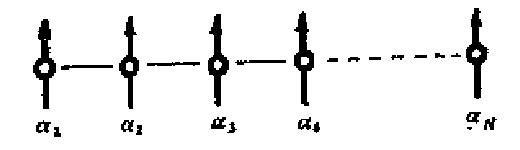
\includegraphics[height=0.50in,width=2.45in,viewport=10 10 600 150,clip]{Figures/Mag_spinwave-0.png}
\caption{\small \textrm{The ground state $|0\rangle$.}}%(与文献\cite{EPJB33-47_2003}图1对比)
\label{Mag_spinwave-0}
\end{figure}
				\item 温度略有升高时,电子自旋有一个发生翻转
\begin{figure}[h!]
\centering
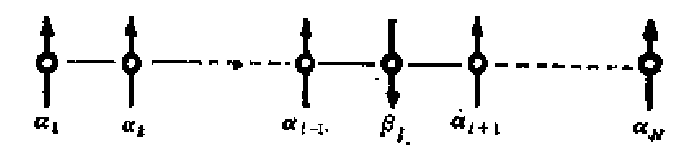
\includegraphics[height=0.50in,width=2.45in,viewport=10 10 680 150,clip]{Figures/Mag_spinwave-1.png}
\caption{\small \textrm{The spin flips at $l$:~ $|l\rangle$.}}%(与文献\cite{EPJB33-47_2003}图1对比)
\label{Mag_spinwave-1}
\end{figure}
			\end{enumerate}
	\end{itemize}
}

\frame
{
	\frametitle{自旋波模型}
	某个格点上出现自旋翻转,\textcolor{blue}{由于相邻格点间存在交换作用,使自旋趋于同向排列}
	\begin{itemize}
		\item \textcolor{red}{翻转的自旋将牵动临近格点自旋,使自趋于翻转}
		\item \textcolor{red}{近邻格点自旋力图驱使翻转的自旋重新翻转过来}
	\end{itemize}
	自旋的翻转不会停留在一个格点,而是以波的形式向周围传播:\\
	\textcolor{blue}{这种自旋翻转在晶体中的传播称为}\textcolor{red}{自旋波(又称磁激子)}
\begin{figure}[h!]
\centering
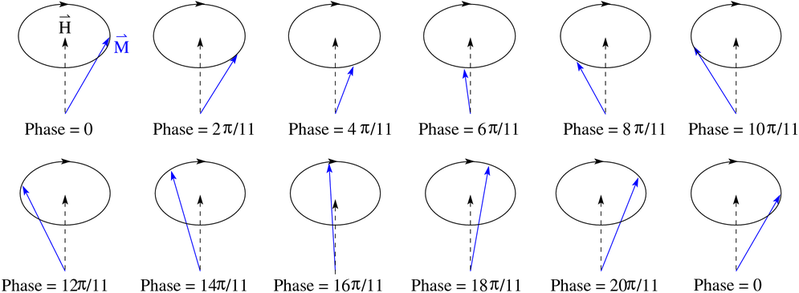
\includegraphics[height=1.15in,width=3.45in,viewport=0 0 830 300,clip]{Figures/Mag_spinwave-2.png}
\caption{\small \textrm{The schematic spin-wave.}}%(与文献\cite{EPJB33-47_2003}图1对比)
\label{Mag_spinwave-2}
\end{figure}
}

\frame
{
	\frametitle{非共线磁矩}
	\begin{itemize}
		\item 研究磁性体系输运时通常只考虑共线磁结构的情况
		\item 真实的物理体系中总会出现非共线的磁结构:\\\textcolor{blue}{特别是在铁磁/非磁金属界面上,铁磁性原子磁矩有可能形成非共线排列}
		\item 最近的研究结果揭示了非共线体系中出现的许多新现象:\\\textcolor{blue}{电流诱导的自旋转矩}\\
			\textcolor{red}{这些非共线的原子磁矩与电子的自旋之间能够通过交换作用,进而引起电子在输运过程中发生自旋翻转,使得自旋向上和自旋向下的输运通道发生了混合,并且处在超导态的非磁金属还能够在铁磁体一侧诱导出长程的自旋三重态配对超导性}
		\item 由于非共线磁结构的引入使得问题变得复杂,目前的实验和理论还并不完备
	\end{itemize}
}

\frame
{
	\frametitle{\textrm{DFT}框架下处理非共线磁矩}
	\textrm{J. K\"ubler}等指出\upcite{JAP63-3482_1988},根据密度泛函理论,当外势是矩阵元为$w^{\alpha\beta}(\vec r)$的$2\times2$矩阵时,令体系的密度矩阵为$\rho^{\alpha\beta}(\vec r)$,则\\
	\textcolor{blue}{体系的电荷密度可以表示为}
	\begin{displaymath}
		Tr[\rho^{\alpha\beta}(r)]\equiv n_{\mathrm{Tr}}(r)=\sum_{\alpha}n^{\alpha\alpha}(\vec r)
	\end{displaymath}
	因此总能量可以表示为
	
	\begin{displaymath}
		\begin{aligned}
			E[\rho^{\alpha\beta}]=&T_0+\sum_{\alpha\beta}\int w^{\alpha\beta}(\vec r)\rho^{\alpha\beta}(\vec r)\mathrm{d}^3r\\
			+&\iint\frac{n_{\mathrm{Tr}}(\vec r^{\prime})n_{\mathrm{Tr}}(\vec r)}{|\vec r-\vec r^{\prime}|}\mathrm{d}^3r\mathrm{d}^3r^{\prime}+E_{\mathrm{XC}}[\rho^{\alpha\beta}]
		\end{aligned}
	\end{displaymath}
}

\frame
{
	\frametitle{\textrm{DFT}框架下处理非共线磁矩}
	\textrm{D. Hobbs~}等\upcite{PRB62-11556_2000}\textcolor{red}{考虑磁化密度的贡献后,将总电荷密度矩阵表示为}
	\begin{displaymath}
		\rho^{\alpha\beta}(\vec r)=\left[n_{\mathrm{Tr}}(\vec r)\delta_{\alpha\beta}+\vec m(\vec r)\vec{\sigma}^{\alpha\beta}\right]/2
	\end{displaymath}
	磁化密度的表示为
	\begin{displaymath}
		\vec m(\vec r)=\sum_{\alpha\beta}\rho^{\alpha\beta}(\vec r)\cdot\vec{\sigma}^{\alpha\beta}
	\end{displaymath}
	其中\textrm{Pauli~}自旋矩阵$\vec{\sigma}=(\sigma_x,\sigma_y,\sigma_z)$定义为
	\begin{displaymath}
		\sigma_x=\left( 
		\begin{matrix}
			0 &1\\
			1 &0
		\end{matrix}
		\right)\quad
		\sigma_y=\left( 
		\begin{matrix}
			0 &-\mathrm{i}\\
			\mathrm{i} &0
		\end{matrix}
		\right)\quad
		\sigma_z=\left( 
		\begin{matrix}
			1 &0\\
			0 &-1
		\end{matrix}
		\right)
	\end{displaymath}
	因此在\textrm{DFT}框架下能量密度泛函可以表示为
	\begin{displaymath}
		E=\sum_{\alpha}\sum_{n}f_n\langle\Psi_n^{\alpha}|-\frac12\nabla^2|\Psi_n^{\alpha}\rangle+E_{\mathrm{H}}[\textcolor{blue}{n_{\mathrm{Tr}}}+n_Z]+E_{\mathrm{XC}}[\textcolor{red}{\rho^{\alpha\beta}}]
	\end{displaymath}
}

\frame
{
	\frametitle{\textrm{DFT}框架下处理非共线磁矩}
	上述表达式中$f_n$是轨道占据数
	
	$E_{\mathrm{H}}[n_{\mathrm{Tr}}+n_Z]$是静电相互作用
	\begin{displaymath}
		E_{\mathrm{H}}[\textcolor{brown}{\rho}]=\frac12\iint\frac{\textcolor{brown}{\rho(\vec r)\rho(\vec r^{\prime})}}{|\vec r-\vec r^{\prime}|}\mathrm{d}\vec r\mathrm{d}\vec r^{\prime}
	\end{displaymath}
	这里$\textcolor{brown}{\rho}=n_{\mathrm{Tr}}+n_Z$

	在\textrm{LSDA}下,交换-相关能泛函表示为
	\begin{displaymath}
		\begin{aligned}
			E_{\mathrm{XC}}[\textcolor{red}{\rho^{\alpha\beta}}]=&\int\textcolor{blue}{n_{\mathrm{Tr}}(\vec r)}\epsilon_{\mathrm{XC}}[\textcolor{red}{\rho^{\alpha\beta}}]\mathrm{d}\vec r\\
			=&\int\textcolor{blue}{n_{\mathrm{Tr}}(\vec r)}\epsilon_{\mathrm{XC}}[\textcolor{blue}{n_{\mathrm{Tr}}(\vec r)},|\vec m(\vec r)|]\mathrm{d}\vec r
		\end{aligned}
	\end{displaymath}
}

\section{\rm{PAW}方法计算非共线磁矩}
\frame
{	
	\frametitle{\textrm{PAW~}方法概要}
	在\textrm{PAW~}方法中,波函数可以表示为
	\begin{displaymath}
		|\Psi_n^{\alpha}\rangle=|\tilde\Psi_n^{\alpha}\rangle+\sum_i(|\phi_i\rangle-|\tilde\phi_i\rangle)\langle \tilde p_i|\tilde\Psi_n^{\alpha}\rangle
	\end{displaymath}
	其中赝波函数用平面波展开
	\begin{displaymath}
		\langle\vec r|\tilde\Psi_n^{\alpha}\rangle=\frac1{\Omega_r^{\frac12}}\sum_{\vec k}C_{n\vec k}^{\alpha}(r)\mathrm{e}^{\mathrm{i}\vec k\cdot\vec r}
	\end{displaymath}
	$\phi$是原子分波,$\tilde\phi$是对应的赝原子分波\\ 
	\vspace*{20pt}
投影子函数$\tilde p_i$与赝原子分波$\tilde\phi_j$正交
$$\langle\tilde p_i|\tilde\phi_j\rangle=\delta_{ij}$$
}

\frame
{	
	\frametitle{\textrm{PAW~}方法的密度矩阵计算}
\textcolor{red}{非共线磁矩的计算中的关键是密度矩阵的处理}
\begin{displaymath}
	n^{\alpha\beta}(\vec r)=\tilde n^{\alpha\beta}+\sideset{^1}{^{\alpha\beta}}n(\vec r)-\sideset{^1}{^{\alpha\beta}}{\tilde n}(\vec r)
\end{displaymath}
这里赝密度矩阵$\tilde n$由倒空间平面波网格上的赝波函数直接计算
\begin{displaymath}
	\tilde n^{\alpha\beta}(\vec r)=\sum_nf_n\langle\tilde\Psi_n^{\beta}|\vec r\rangle\langle\vec r|\tilde\Psi_n^{\alpha}\rangle
\end{displaymath}
在位密度矩阵$\sideset{^1}{}n$和$\sideset{^1}{}{\tilde n}$分别原子球截断半径$r_{\mathrm{rad}}$内计算
\begin{displaymath}
	\begin{aligned}
		\sideset{^1}{^{\alpha\beta}}n(\vec r)=&\sum_{i,j}\rho_{ij}^{\alpha\beta}\langle\phi_i|\vec r\rangle\langle\vec r|\phi_j\rangle\\
		\sideset{^1}{^{\alpha\beta}}{\tilde n}(\vec r)=&\sum_{i,j}\rho_{ij}^{\alpha\beta}\langle\tilde\phi_i|\vec r\rangle\langle\vec r|\tilde\phi_j\rangle 
	\end{aligned}
\end{displaymath}
这里$\rho_{ij}^{\alpha\beta}$的计算由下式给出
\begin{displaymath}
	\rho_{ij}^{\alpha\beta}=\sum_nf_n\langle\tilde\Psi_n^{\beta}|\tilde p_i\rangle\langle\tilde\rho_j|\tilde\Psi_n^{\alpha}\rangle
\end{displaymath}
}

\frame
{
	\frametitle{补偿电荷密度的影响}
	补偿电荷密度$\hat n$要求$\sideset{^1}{}{\tilde n}+\hat n$与$\sideset{^1}{}n$具有相同的多极矩,即要求
	\begin{displaymath}
		\int_{\Omega_r}\left[ \sideset{^1}{^{\alpha\beta}}n(\vec r)-\sideset{^1}{^{\alpha\beta}}{\tilde n}(\vec r)-\hat n^{\alpha\beta}(\vec r) \right]|\vec r-\vec R|^lY_L^{\ast}(\widehat{\vec r-\vec R})\mathrm{d}\vec r=0
	\end{displaymath}
	补偿电荷密度$\hat n^{\alpha\beta}(\vec r)$由多极矩计算
	\begin{displaymath}
		\begin{aligned}
			\hat n^{\alpha\beta}(\vec r)&=\sum_{(i,j),L}\rho_{ij}^{\alpha\beta}\hat Q_{ij}^L(\vec r)\\
			\hat Q_{ij}^L(\vec r)&=q_{ij}^Lg_l(|\vec r-\vec R|)Y_L(\widehat(\vec r-\vec R))
		\end{aligned}
	\end{displaymath}
其中
\begin{displaymath}
	\begin{aligned}
		q_{ij}^L=&\int_{\Omega_r}Q_{ij}(\vec r)|\vec r-\vec R|^lY_L^{\ast}(\widehat{\vec r-\vec R})\mathrm{d}\vec r\\
		Q_{ij}(\vec r)=&\phi_i^{\ast}(\vec r)\phi_j(\vec r)-\tilde\phi_i^{\ast}(\vec r)\tilde\phi_j(\vec r)
	\end{aligned}
\end{displaymath}
}

\frame
{
	\frametitle{总能量泛函的表示}
	\vspace*{-10pt}\textrm{PAW~}方法的总能量泛函计算
	$$E=\tilde E+E^1+\tilde E^1$$
	各项的表达式为
	\begin{displaymath}
		\begin{aligned}
			\tilde E=&\sum_{\alpha}\sum_nf_n\langle\tilde\Psi_n^{\alpha}|-\frac12\nabla^2|\tilde\Psi_n^{\alpha}\rangle+E_{\textrm{XC}}[\tilde n^{\alpha\beta}+\hat n^{\alpha\beta}+\tilde n_c]\\
			&+E_{\mathrm{H}}[\tilde n_{\mathrm{Tr}}+\hat n_{\mathrm{Tr}}]+\int v_{\mathrm H}[\tilde n_{Zc}](\vec r)[\tilde n_{\mathrm{Tr}}(\vec r)+\hat n_{\mathrm{Tr}}(\vec r)]\mathrm{d}\vec r+U(\vec R,Z_{\mathrm{ion}})
		\end{aligned}
	\end{displaymath}
\vspace*{-6pt}
	\begin{displaymath}
		\begin{aligned}
			\tilde E^1=&\sum_{\alpha\beta}\sum_{(i,j)}\rho_{ij}^{\alpha\beta}\langle\tilde\phi_i^{\alpha}|-\frac12\nabla^2|\tilde\phi_j^{\alpha}\rangle+\overline{E_{\textrm{XC}}[\sideset{^1}{^{\alpha\beta}}{\tilde n}+\hat n^{\alpha\beta}+\tilde n_c]}\\
			&+\overline{E_{\mathrm{H}}[\sideset{^1}{_{\mathrm{Tr}}}{\tilde n}+\hat n_{\mathrm{Tr}}]}+\int_{\Omega_r}v_{\mathrm H}[\tilde n_{Zc}](\vec r)[\sideset{^1}{_{\mathrm{Tr}}}{\tilde n}(\vec r)+\hat n_{\mathrm{Tr}}(\vec r)]\mathrm{d}\vec r
		\end{aligned}
	\end{displaymath}
\vspace*{-3pt}
	\begin{displaymath}
		\begin{aligned}
			E^1=&\sum_{\alpha\beta}\sum_{(i,j)}\rho_{ij}^{\alpha\beta}\langle\phi_i^{\alpha}|-\frac12\nabla^2|\phi_j^{\alpha}\rangle+\overline{E_{\textrm{XC}}[\sideset{^1}{^{\alpha\beta}}n+n_c]}\\
			&+\overline{E_{\mathrm{H}}[\sideset{^1}{_{\mathrm{Tr}}}n]}+\int_{\Omega_r}v_{\mathrm H}[n_{Zc}](\vec r)[\sideset{^1}{_{\mathrm{Tr}}}n(\vec r)]\mathrm{d}\vec r
		\end{aligned}
	\end{displaymath}
}

\frame
{
	\frametitle{静电势函数和重叠矩阵}
	\begin{itemize}
		\item 静电势$v_{\mathrm H}[\rho](\vec r)$定义为
	\begin{displaymath}
		v_{\mathrm H}[\rho](\vec r)=\int\frac{\rho(\vec r^{\prime})}{|\vec r-\vec r^{\prime}|}\mathrm{d}\vec r^{\prime}
	\end{displaymath}
		\item \textrm{PAW~}方法的赝波函数$\tilde\Psi_n^{\alpha}$构成的重叠矩阵满足广义正交条件
			\begin{displaymath}
				\sum_{\alpha}\langle\tilde\Psi_n^{\alpha}|S^{\alpha\alpha}|\tilde\Psi_m^{\alpha}\rangle=\delta_{nm}
			\end{displaymath}
			这里\textcolor{blue}{重叠矩阵}定义为
			\begin{displaymath}
				S^{\alpha\beta}[\{\vec R\}]=\delta_{\alpha\beta}\left( 1+\sum_i|\tilde p_i\rangle q_{ij} \langle\tilde p_j| \right)
			\end{displaymath}
			这里$q_{ij}$表达式为
			\begin{displaymath}
				q_{ij}=\langle\phi_i|\phi_j\rangle-\langle\tilde\phi_i|\tilde\phi_j\rangle=\int_{\Omega_r}Q_{ij}(\vec r)\mathrm{d}\vec r=\sqrt{4\pi}q_{ij}^0
			\end{displaymath}

	\end{itemize}

}

\frame
{
	\frametitle{\textrm{Hamiltonian}矩阵}
	为得到\textrm{Hamiltonian}矩阵,定义\textcolor{red}{赝电荷密度算符}
	\begin{displaymath}
		\tilde\rho^{\alpha\beta}=\sum_nf_n|\tilde\Psi_n^{\alpha}\rangle\Psi_n^{\beta}|
	\end{displaymath}
	由\textrm{Hamiltonian}算符定义
	\begin{displaymath}
		\frac{\mathrm{d}E}{\mathrm{d}\tilde\rho^{\alpha\beta}}=H^{\alpha\beta}
	\end{displaymath}
	\textcolor{red}{注意}:~$\tilde\rho^{\alpha\beta}$对\textcolor{blue}{动能项}、\textcolor{blue}{赝电荷密度$\tilde n_{\mathrm{Tr}}$}、\textcolor{blue}{赝磁化密度$\tilde{\vec m}$}和\textcolor{blue}{缀加电荷占据数$\rho_{ij}^{\alpha\beta}$}都有贡献,因此总能量的变分可以写成
	\vspace*{-5pt}
	\begin{displaymath}
		\begin{aligned}
			\frac{\mathrm{d}E}{\mathrm{d}\tilde\rho^{\alpha\beta}}=&\frac{\partial E}{\partial\tilde\rho^{\alpha\beta}}+\int\frac{\delta E}{\delta\tilde n_{\mathrm{Tr}}(\vec r)}\underbrace{\frac{\partial\tilde n_{\mathrm{Tr}}(\vec r)}{\partial\tilde\rho^{\alpha\beta}}}_{|\vec r\rangle\langle\vec r|}\mathrm{d}\vec r\\
			+&\int\underbrace{\frac{\delta E}{\delta\tilde{\vec m}(\vec r)}}_{\vec b}\underbrace{\frac{\partial\tilde{\vec m}(\vec r)}{\partial\tilde\rho^{\alpha\beta}}}_{|\vec r\rangle\vec\sigma\langle\vec r|}\mathrm{d}\vec r+\sum_{(i,j)}\frac{\partial E}{\partial\rho_{ij}^{\alpha\beta}}\underbrace{\frac{\partial\rho_{ij}^{\alpha\beta}}{\partial\tilde\rho^{\alpha\beta}}}_{|\tilde p_i\rangle\langle p_j|}
		\end{aligned}
	\end{displaymath}
}

\frame
{
	\frametitle{\textrm{Hamiltonian}矩阵}
	\begin{itemize}
		\item \textcolor{blue}{对$\tilde\rho^{\alpha\beta}$的偏导}是\textcolor{red}{动能算符$-\frac12\nabla^2\delta_{\alpha\beta}$}
		\item \textcolor{blue}{对$\tilde n_{\mathrm{Tr}}(\vec r)$和$\tilde{\vec m}(\vec r)$的偏导}是\textcolor{red}{有效单电子势$\tilde v_{\mathrm{eff}}^{\alpha\beta}(\vec r)$}(\textcolor{brown}{$2\times2$矩阵})
			\begin{displaymath}
				\begin{aligned}
					\tilde v_{\mathrm{eff}}^{\alpha\beta}[\tilde n](\vec r)=&v_{\mathrm{H}}[\tilde n_{\mathrm{Tr}}+\hat n_{\mathrm{Tr}}+\tilde n_{Zc}](r)\delta_{\alpha\beta}\\
					+&v_{\mathrm{XC}}[\tilde n^{\alpha\beta}+\hat n^{\alpha\beta}+\tilde n_c](\vec r)\delta_{\alpha\beta}\\
					+&\vec b[\tilde n^{\alpha\beta}+\hat n^{\alpha\beta}+\tilde n_c](\vec r)\cdot\vec{\sigma}^{\alpha\beta}
				\end{aligned}
			\end{displaymath}
		\item 在\textrm{LSDA}近似下,\textcolor{red}{交换-相关势的非磁性部分贡献}
			\begin{displaymath}
				\begin{aligned}
					v_{\mathrm{XC}}[n^{\alpha\beta}](\vec r)=&\frac{\delta E_{\mathrm{XC}}[n^{\alpha\beta}]}{\delta n_{\mathrm{Tr}}(\vec r)}\\
					=&\epsilon_{\mathrm{XC}}[n^{\alpha\beta}(\vec r)]+n_{\mathrm{Tr}}(\vec r)\frac{\partial\epsilon_{\mathrm{XC}}[n^{\alpha\beta}(\vec r)]}{\partial n_{\mathrm{Tr}}(\vec r)}
				\end{aligned}
			\end{displaymath}
	\end{itemize}
}

\frame
{
	\frametitle{\textrm{Hamiltonian}矩阵}
	\begin{itemize}
			\textcolor{red}{交换-相关的磁性部分贡献}
			\begin{displaymath}
				\begin{aligned}
					\vec b[n^{\alpha\beta}](\vec r)=&\frac{\delta E_{\mathrm{XC}}[n^{\alpha\beta}]}{\delta\vec m(\vec r)}\\
					&=\frac{\partial|\vec m(\vec r)|}{\partial{\vec m}(\vec r)}\frac{\delta E_{\mathrm{XC}}[n^{\alpha\beta}(\vec r)]}{\partial|\vec m(\vec r)|}\\
					&=\hat m(\vec r)n_{\mathrm{Tc}}(\vec r)\frac{\partial\epsilon_{\mathrm{XC}}[n^{\alpha\beta}(\vec r)]}{\partial\vec m(\vec r)}
				\end{aligned}
			\end{displaymath}
			其中$$\hat m(\vec r)=\frac{\partial|\vec m(\vec r)|}{\partial\vec m(\vec r)}$$
			是$\vec r$点的磁化密度方向

			\textcolor{red}{$\vec b(\vec r)$与磁化密度$\vec m(\vec r)$处处平行}
	\end{itemize}
}

\frame
{
	\frametitle{\textrm{Hamiltonian}矩阵}
	\begin{itemize}
		\item \textcolor{red}{能量$\tilde E$中,缀加电荷占据数$\rho_{ij}^{\alpha\beta}$只对补偿电荷$\hat n$有贡献},因此
			\begin{displaymath}
				\begin{aligned}
					\hat D_{ij}^{\alpha\beta}=&\frac{\partial\tilde E}{\partial\rho_{ij}^{\alpha\beta}}=\int\frac{\delta\tilde E}{\delta\hat n^{\alpha\beta}(\vec r)}\frac{\partial\hat n^{\alpha\beta}(\vec r)}{\partial\rho_{ij}^{\alpha\beta}}\mathrm{d}\vec r\\
					=&\sum_L\int\tilde v_{\mathrm{eff}}^{\alpha\beta}(\vec r)\hat Q_{ij}^L(\vec r)\mathrm{d}\vec r
				\end{aligned}
			\end{displaymath}
			\textcolor{blue}{因为赝波函数$\tilde Psi_n^{\alpha}$对应的电荷密度分布与真实波函数$\Psi_n^{\alpha}$的电荷密度多极矩不同,$\hat D_{ij}^{\alpha\beta}$修正了波函数$\tilde\Psi_n^{\alpha}$的长程行为}
	\end{itemize}
}

\frame
{
	\frametitle{\textrm{Hamiltonian}矩阵}
	\begin{itemize}
		\item \textcolor{red}{能量$E^1$和$\tilde E^1$中只有$\rho_{ij}^{\alpha\beta}$有贡献},因此
			\begin{displaymath}
				\sideset{^1}{_{ij}^{\alpha\beta}}D=\frac{\partial E^1}{\partial\rho_{ij}^{\alpha\beta}}=\langle\phi_i|-\frac12\nabla^2\delta_{\alpha\beta}+\sideset{^1}{_{\mathrm{eff}}^{\alpha\beta}}v|\phi_j\rangle
			\end{displaymath}
			这里
			\begin{displaymath}
				\begin{aligned}
					\sideset{^1}{_{\mathrm{eff}}^{\alpha\beta}}v[\sideset{^1}{}n](\vec r)=&v_{\mathrm{H}}[\sideset{^1}{_\mathrm{Tr}}n+n_{\mathrm{Zc}}](\vec r)\delta_{\alpha\beta}\\
					+&v_{\mathrm{XC}}[\sideset{^1}{^{\alpha\beta}}n+n_c](\vec r)\delta_{\alpha\beta}\\
					+&\vec b[\sideset{^1}{^{\alpha\beta}}n+n_c](\vec r)\cdot\vec{\sigma}^{\alpha\beta}
				\end{aligned}
			\end{displaymath}
	\end{itemize}
}

\frame
{
	\frametitle{\textrm{Hamiltonian}矩阵}
	\begin{itemize}
		\item 对$\tilde E^1$类似可得
			\begin{displaymath}
				\begin{aligned}
					\sideset{^1}{_{ij}^{\alpha\beta}}{\tilde D}=&\frac{\partial\tilde E^1}{\partial\rho_{ij}^{\alpha\beta}}=\langle\tilde \phi_i|-\frac12\nabla^2\delta_{\alpha\beta}+\sideset{^1}{_{\mathrm{eff}}^{\alpha\beta}}{\tilde v}|\tilde\phi_j\rangle\\
					+&\sum_L\int_{\Omega_r}\sideset{^1}{_{\mathrm{eff}}^{\alpha\beta}}{\tilde v}(\vec r)\hat Q_{ij}^L(\vec r)\mathrm{d}\vec r
				\end{aligned}
			\end{displaymath}
			\textcolor{blue}{第一项源自$\sideset{^1}{}{\tilde n}$对$\rho_{ij}^{\alpha\beta}$的变分,第二项源自$\hat n$对$\rho_{ij}^{\alpha\beta}$}
			其中
			\begin{displaymath}
				\begin{aligned}
					\sideset{^1}{_{\mathrm{eff}}^{\alpha\beta}}{\tilde v}[\sideset{^1}{}n](\vec r)=&v_{\mathrm{H}}[\sideset{^1}{_\mathrm{Tr}}{\tilde n}+\hat n_{\mathrm{Tr}}+\tilde n_{\mathrm{Zc}}](\vec r)\delta_{\alpha\beta}\\
					+&v_{\mathrm{XC}}[\sideset{^1}{^{\alpha\beta}}{\tilde n}+\hat n^{\alpha\beta}+\tilde n_c](\vec r)\delta_{\alpha\beta}\\
					+&\vec b[\sideset{^1}{^{\alpha\beta}}{\tilde n}+\hat n^{\alpha\beta}+\tilde n_c](\vec r)\cdot\vec{\sigma}^{\alpha\beta}
				\end{aligned}
			\end{displaymath}
	\end{itemize}
}

\frame
{
	\frametitle{\textrm{Hamiltonian}矩阵}
	最后得到\textrm{Hamiltonian}的表达式
	\begin{displaymath}
		\begin{aligned}
			H^{\alpha\beta}[n,\{\vec R\}]=&-\frac12\nabla^2\delta_{\alpha\beta}+\tilde v_{\mathrm{eff}}^{\alpha\beta}\\
			+&\sum_{(i,j)}|\tilde p_i\rangle(\sideset{^1}{_{ij}^{\alpha\beta}}D+\hat D_{ij}^{\alpha\beta}-\sideset{^1}{_{ij}^{\alpha\beta}}{\tilde D})\langle\tilde p_j|
		\end{aligned}
	\end{displaymath}
	其中
	\begin{displaymath}
		\hat D_{ij}^{\alpha\beta}=\sum_{(i,j),L}\langle\tilde\Psi_n^{\beta}|\tilde p_i\rangle\langle\tilde p_j|\Psi_n^{\alpha}\rangle\int\tilde v_{\mathrm{eff}}^{\alpha\beta}(\vec r)\hat Q_{ij}^L(\vec r)\mathrm{d}\vec r
	\end{displaymath}
	\textcolor{red}{描述的是单个电子的补偿电荷密度与单电子有效势的相互作用(属于长程静电相互作用)}

	基于赝波函数的广义\textrm{Kohn-Sham}方程
	\begin{displaymath}
		\sum_{\beta}H^{\alpha\beta}|\tilde\Psi_n^{\beta}\rangle=\varepsilon_nS^{\alpha\alpha}|\Psi_n^{\alpha}\rangle
	\end{displaymath}
}

%\frame
%{
%\frametitle{发展统一理论框架下的材料计算程序}
%\begin{itemize}
%	\item
%\end{itemize}
%}

\appendix
%------------------------------------------------------------------------Reference----------------------------------------------------------------------------------------------
%\begin{thebibliography}{99}
%-----------------------------------------------------------------------------------------------------------------------------------------------------------------------%
%\frame
%{
%\frametitle{主要参考文献}
%{\small
%\bibitem{Singh_Book}\textrm{D. J. Singh. \textit{Plane Wave, PseudoPotential and the LAPW method} (Kluwer Academic, Boston,USA, 1994)}					%
%  \nocite{*}																				%
%}
%}
%\end{thebibliography}
\begin{thebibliography}{99}
\frame
{
\frametitle{主要参考文献}
{\small
%	\bibitem{Huang_Han}黄昆\:原著、韩汝琦\:改编, {\textit{固体物理学}}\:高等教育出版社, 北京, 1988
%	\bibitem{Xie_Lu}谢希德、陆栋\:主编, {\textit{固体能带理论}}\:复旦大学出版社, 上海, 1998
	\bibitem{JAP63-3482_1988}\textrm{J. K\"ubler, K. H. H\"ock and J. Sticht. \textit{J. Appl. Phys.}, \textbf{63} (1988), 3482}
	\bibitem{Novak}\textrm{P. Nov$\mathrm{\acute a}$k. \textit{Calculation of spin-orbit coupling} (unpublished)}
	\bibitem{Dai_Qian}戴道生,钱昆明, {\textit{铁磁学}}(上册),\:科学出版社, 北京, 1998
	\bibitem{JPCSSP13-2675_1980}\textrm{A. H. MacDonald, W. E. Pickett and D. D. Koelling. \textit{J. Phys. C: Solid St. Phys.}, \textbf{13} (1980), 2675}
	\bibitem{PRB62-11556_2000}\textrm{D. Hobbs, G. Kresse and J. Hafner. \textit{Phys. Rev.} B, \textbf{62} (2000), 11556}
}
\nocite*{}
}
\end{thebibliography}
%{\small
%\phantomsection\addcontentsline{toc}{section}{Bibliography}	 %直接调用\addcontentsline命令可能导致超链指向不准确,一般需要在之前调用一次\phantomsection命令加以修正	%
%\bibliography{Myref}																			%
%\bibliographystyle{mybib}																		%
%  \nocite{*}																				%
%}
%-----------------------------------------------------------------------------------------------------------------------------------------------------------------------%


%-----------------------------------------------------------Beamer下不建议使用bib,因为涉及分页--------------------------------------------------------------------------%
%{\small
%\phantomsection\addcontentsline{toc}{section}{Bibliography}	 %直接调用\addcontentsline命令可能导致超链指向不准确,一般需要在之前调用一次\phantomsection命令加以修正	%
%\bibliography{Myref}																			%
%\bibliographystyle{mybib}																		%
%  \nocite{*}																				%
%}

%------------------------------------------------------------------------------------------------------------------------------------------------------------------------------%

%-------------------------------------------------------------------------Thanks------------------------------------------------------------------------------------------------
%\section{致谢}
%\frame
%{
%\frametitle{致$\quad$谢}
%\begin{itemize}
%    \setlength{\itemsep}{20pt}
%  \item 感谢本团队高兴誉、吴泉生、宋红州等各位老师参与的讨论
%  \item 感谢莫所长、宋主任以及软件中心各位老师和同事
%  \item 感谢王崇愚先生的帮助
%\end{itemize}
%}

\logo{}									%不显示logo
\frame
{
\vskip 60 pt
%\hskip 10pt \textcolor{blue}{\Huge 感谢答辩委员会各位老师\,\textrm{!}}\\
\vskip 35 pt
\hskip 60pt \textcolor{blue}{\Huge 谢谢大家\:!}
%\vskip 15 pt
%\hskip 40pt \textcolor{blue}{\Huge \textrm{for your attention\:!}}
}

%-------------------------------------------------------------------------------------------------------------------------------------------------------------------------------

\clearpage
%\end{CJK*}
\end{document}
